\documentclass{article}
\usepackage{graphicx}
\usepackage{hyperref}
\hypersetup{
    colorlinks=true,
    linkcolor=blue,
    filecolor=magenta,      
    urlcolor=cyan,
    pdftitle={Overleaf Example},
    pdfpagemode=FullScreen,
}
\usepackage{array}
\usepackage{titlesec}
\usepackage{geometry}
 \geometry{
 a4paper,
 total={170mm,257mm},
 left=20mm,
 top=20mm,
 }
\graphicspath{ {./images/} }

\begin{document}

\title{Unit 15 M2}
\author{Chris}
\date{}
\maketitle
 

\section{Build \& test a prototype – P5}

\underline{Strings} are traditionally sequences of characters. In our games, they are used for names in the HUD and the main menu. \underline{Inputs} refer to any data or information sent to a computer for processing. User input, delivered through input devices, consists of hardware inputs from players. This typically includes key presses, mouse clicks, mouse movements, controller button presses, or joystick movements. Examples of input devices include:
\begin{enumerate}
	\item Keyboard
	\item Mouse
	\item Microphone
	\item Webcam
\end{enumerate}
\underline{Output} devices enhance user interaction with computer systems by converting data signals into forms that are more comprehensible to humans, such as visuals or audio. These devices enable users to transform data into the most suitable format for specific situations, thereby improving data accessibility and the ability of users or audiences to recall it accurately. Examples of output devices include:
\begin{enumerate}
	\item Braille reader
	\item Computer speakers
	\item GPS
	\item Headphones
\end{enumerate}
The \underline{selection} available for our games becomes accessible upon launching the game. For \underline{iteration}, the prototype will utilize this process to quickly enhance the game and meet our client's requirements. Iteration involves repeatedly proposing, prototyping, playtesting, and reevaluating a video game before its final release. \underline{Subroutines} are comprised of a collection of public static methods that simplify the management of conditional events and routines. \newline


We utilize numerous \underline{conditional} statements in our game. For instance, when a player dies, their health bar resets to zero. Another scenario involves the player entering a trap's hit box, triggering the spawn of five kunai in five different directions. We use \underline{counting} mechanisms to tally the player's score. \underline{Totaling}, scoring in our game involves maintaining an integer that increments each time the player collects an item, which adds to the total score displayed on the scoreboard. In recent years, there has been a shift in \underline{data structures} towards data-oriented design, which emphasizes high-performance computing. This method enhances CPU cache efficiency and optimizes memory usage, maximizing the performance capabilities of modern CPUs.

\section{Test data}
\begin{center}		                               
	\begin{tabular}{|m{1em}|m{3em}|m{20em}|m{5em}|m{1.25em}|m{10em}|}
	\hline
		n & Test Case & Expected Result & Actual Result & P/F & Verified  \\
	\hline
	\hline
		1 & Player spawns & The Player Character Spawns in the correct spot & The character spawned in correctly & p & 
\includegraphics[scale=0.5]{Player spawns} \\
	\hline
		2 & Falling Platform & When the player touches the platform, the platform falls  & The platform fell & p & 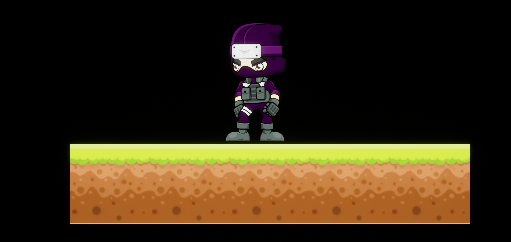
\includegraphics[scale=0.25]{Falling plat}\\
	\hline
		3 & Moving Platform & When the level loads the moving platform starts moving right then back to left  & the platform on the level open starts moving  & p & 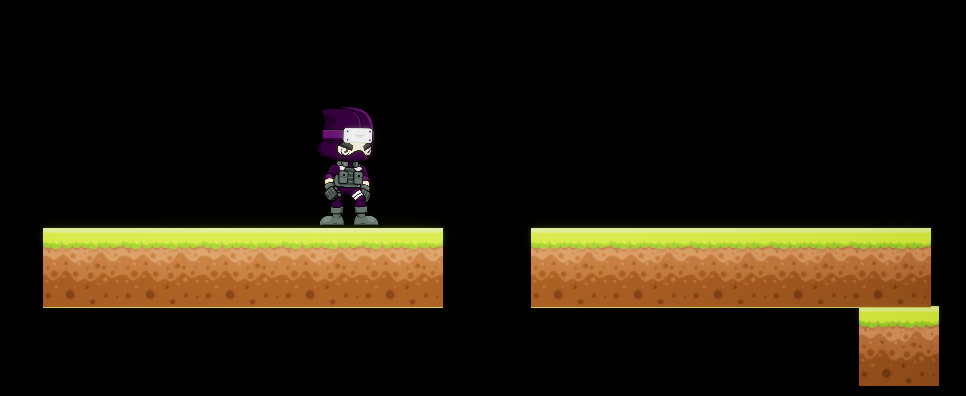
\includegraphics[scale=0.15]{Capture} \\
	\hline
		4 & Health pickup  & When the player touches the health pickup there health increase & The player touched the health pickup and there health increase & p & 
\includegraphics[scale=0.75]{health 1} \\
	\hline
\end{tabular}
\end{center}

\section{Black box}
The box testing takes advantage of extensive knowledge of an application’s internals to develop highly-targeted test cases. Examples of tests that might be performed during white box testing include. What is black box testing is a method of software testing that examines the functionality of an application without peering into its internal structures or workings. This method of test can be applied virtually to every level of software testing: unit, integration, system and acceptance. Black-box testing is also used as a method in penetration testing, where an ethical hacker simulates an external hacking or cyber warfare attack with no knowledge of the system being attacked. 

Black box testing involves testing a system with no prior knowledge of its internal workings. A tester provides an input, and observes the output generated by the system under test. This makes it possible to identify how the system responds to expected and unexpected user actions, its response time, usability issues and reliability issues.

Advantages of Black Box Testing

The tester does not need to have more functional knowledge or programming skills to implement the Black Box Testing.
It is efficient for implementing the tests in the larger system.
Tests are executed from the user’s or client’s point of view.
Test cases are easily reproducible.
It is used to find the ambiguity and contradictions in the functional specifications.

Disadvantages of Black Box Testing

There is a possibility of repeating the same tests while implementing the testing process.
Without clear functional specifications, test cases are difficult to implement.
It is difficult to execute the test cases because of complex inputs at different stages of testing.
Sometimes, the reason for the test failure cannot be detected.
Some programs in the application are not tested.
It does not reveal the errors in the control structure.
Working with a large sample space of inputs can be exhaustive and consumes a lot of time.

\section{White box}
White box testing takes advantage of extensive knowledge of an application's internals to develop highly-targeted test cases. Examples of tests that might be performed during white box testing include

\begin{enumerate}
	\item Path checking: White box testing enables the examination of different execution paths within an application to verify the accuracy, relevance, and effectiveness of all conditional statements.
	\item Output Validation: This process lists the diverse potential inputs to a function and confirms that each one yields the anticipated outcome.
	\item Security Testing: Static code analysis and additional white box testing methods are employed to pinpoint possible vulnerabilities within an application and verify its adherence to secure development standards.
	\item Loop: Testing: Evaluates the loops in an application to confirm their accuracy, efficiency, and proper management of the variables in their scope 
	\item Data Flow Testing: Monitors variables across a program's execution paths to verify that they are declared, initialized, utilized, and correctly manipulated.
\end{enumerate}

White box testing can be performed for few different purpose. The three types of white box testing are:
\begin{enumerate}
	\item Unit Testing
	\item Integration Testing
	\item Regression Testing
\end{enumerate}

\section{Alpha}
In this stage of game testing, the game remains under development, and parallel testing is conducted to ensure it is being developed without glitches and operates smoothly without crashing. Extensive documentation of hardware and software factors is required during this phase to integrate these elements effectively at earlier stages.

\section{Beta}
During beta testing, the game is nearly production-ready yet still has significant issues to resolve. In this phase, game testers are required to thoroughly explore all potential ways to break the game and identify any minor issues.

\section{User testing}
User testing in game development refers to the process where actual users are invited to test the game in a stage close to it's release. The goal is to gather feedback on  the game's usability, functionality, and overall player experience. This helps developers understand how players interact with the game, identify any confusing elements, and assess the game's enjoyment level.



\end{document}
